%\documentstyle[12pt,vita,fullpage]{article}
\documentclass[10pt]{article}

\usepackage{vita}
%\usepackage{myfullpage}
\usepackage{fullpage}
\usepackage{graphicx}

\setlength{\parindent}{0em}

\title{Curriculum Vita}
\author{Wayne O. Cochran\\
       Clinical Assistant Professor of Computer Science\\
       School of Engineering and Computer Science\\
       Washington State University Vancouver\\
       14204 NE Salmon Creek Avenue\\
       Vancouver, WA 98686-9600\\
       (360) 546-9463\\
       {\tt wcochran@vancouver.wsu.edu} \\
       {\tt http://ezekiel.vancouver.wsu.edu/\~{}wayne}}

\begin{document}

\maketitle

%\noindent{\large\bf Current Appointment}\\

%Clinical Assistant Professor in the the School of
%Engineering and 
%Computer Science at Washington State University Vancouver. 
%%Appointment began in August, 1999.

%\vspace{0.5cm}

\noindent{\large\bf Research and Technical Interests}\\

{\em Computer Graphics, Geometric Modeling, Rasterization, Real-Time Rendering
and GPU Programming.}
My career in computer graphics started by 
implementing rasterization firmware
for industrial graphics boards based on
TI's TMS34010 line of graphics processors.
Later I developed a 3D rendering system
that used the TMS34082 floating  point coprocessor.
Essentially I was programming GPU's long before
the current wave of GPU coding become popular.
Later, during graduate school, I developed an interest
in a class of fractal models that were used for compressing
images at unusually high bit rates. I extended these
algorithms (along with methods based on the DCT)
to compress 3-D volumetric data produced by CT
and MRI machines. Following this, I developed a variety of methods
based on fractal interpolation functions to model
and render intricate curves and surfaces.
I remain interested in modeling 
complex surfaces and textures with fractals and I am
investigating techniques inspired by
Wang Tiles to generate infinitely detailed structures.
Due to the availability of cheap video hardware,
GPU programming
has now extended beyond the realm of computer graphics.
General Purpose GPU (GPGPU) techniques are also
an interest of mine.
I enjoy programming Apple's mobile devices, the iPad and iPhone,
which utilize embedded GPU's.

\vspace{0.5cm}

%\noindent{\large\bf Education}\\[2ex]
\noindent{\large\bf Education}

\begin{itemize}
\item {\bf Ph.D.} Computer Science, 1998,
Washington State University. \\
%School of Electrical Engineering and Computer Science.
Dissertation Title: ``A Recurrent Modeling Toolset.''
%Advisor: John C. Hart.
%GPA: 3.98. 

\item {\bf M.S.} Computer Science, 1994,
Washington State University. \\
%School of Electrical Engineering and Computer Science.
Thesis title: ``Fractal Volume Compression.''
%Advisor: John C. Hart.
%GPA: 4.00.

\item {\bf B.S.} Mathematics, cum laude, 1990.
% College of Arts and Sciences,
University of Washington. 
%GPA: 3.75.
\end{itemize}

\vspace{0.25cm}

%\pagebreak

%\begin{itemize}
%\item Computer Graphics
%  \begin{itemize}
%  \item Rendering  
%  \end{itemize}
%\item Geometric Modeling
%  \begin{itemize}
%  \item Modeling Complex Geometry
%  \end{itemize}
%\item Scientific Visualization
%  \begin{itemize}
%  \item Volume Visualization
%  \item Volume Data Compression
%  \end{itemize}
%\end{itemize}

\noindent{\large\bf Professional Experience}

\begin{itemize}

\item {\bf Clinical Assistant Professor}, 1999-present,
Washington State University Vancouver.
My original position was on a tenure track, but was later switched
to a clinical position to match teaching interests.
Courses taught at WSUV:
{\em Mobile Application Development, Programming Tools, 
Automata and Formal Languages, 
Numerical Computing,
Programming Language Design,
Operating Systems and Computer Architecture, 
Introduction to Computer Graphics,
Advanced Computer Graphics, Theory of Computation} and {\em Compiler Design.}
I am heavily involved in program development for 
the computer science program which started in the fall of 1999.
Research involves intricate surface and texture
modeling using recurrent models and Wang Tiles.
I also have high interest in OpenGL and GPU programming for both
graphical applications and general purpose parallel computing.

\item {\bf Instructor}, 1998-1999,
Washington State University. I performed research and taught
courses in Introduction to Microprocessors, C Programming,
Windows Programming, Computer Networks, and Java Programming.

\item {\bf Research Assistant}, 1994-1998,
Washington State University.
My research included volumetric compression using fractals,
and other techniques using fractals to model complex geometry
({\it e.g.,} rough curves and surfaces). Research was part of the
{\em Recurrent Modeling Project} funded by Intel and a grant
from the NSF.
%Also acted as substitute teacher for Computer Graphics, 
%Advanced Computer Graphics, and Numerical Computing. 

\item {\bf Research/Teaching Assistant}, 1992--1994, 
Washington State University.
Contributed research for and implementation of knowledge based systems.
Lab instructor for
introductory computer programming courses.

\item {\bf Software Engineer}, 1990-1992,
Raster Graphics Inc
(assets acquired by Peritek Corporation in 2001)
{\tt http://www.rastergraf.com}
1804-P SE First St.
Redmond, Oregon 97756
% 1804 SE First Street
%Redmond, OR 97756.
(541) 923-5530
Job Overview: 
Design and implementation of rasterization firmware for
industrial graphics boards. Design and implementation of
3D rendering libraries.
\end{itemize}

%\vspace{0.25cm}

%\pagebreak

%\noindent{\large\bf Current Research Overview}

%\begin{enumerate}
%\item Recurrent surfaces\\
%Fractals have been used for decades for creating amazingly detailed and %complex images. In most situations, these images do not represent any known %target shape, but are simply created for their mathematical intricacy and %beauty. In other cases, fractals have been used to model the patterns found %in marble, the texture of tree bark, and alien landscapes. The algorithms %that generate these shapes are nondeterministic, meaning that only the %general character of the target shape is specified, whereas the specific %details are controlled somehow through random number generation. The focus of %my research involves constructing deterministic fractal models that can %approximate known target shapes both in character and in specific detail. 
%%Recurrent Interpolation Surfaces (RIS), a class of 
%%fractal surfaces I have constructed, are appropriate for 
%%modeling intricate terrain data. The surface is defined by 
%%a function whose graph is the attractor of an Iterated 
%%Function System (IFS). 
%%The images
%%below are examples of the types of intricate surfaces that
%%can be generated using this model.
%%This function is constrained to interpolate a known set of 
%%surface elevation values that can be retrieved from 
%% digitial elevation maps of known mountain ranges. Each of the 
%%\begin{center}
%%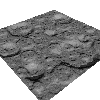
\includegraphics[width=2in]{moon.pdf}
%%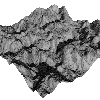
\includegraphics[width=2in]{mts.pdf}
%%\end{center}

%\item Automatic and procedural creation of Wang Tiles\\
%Wang Tiles allow for efficient (real time) 
%aperiodic tiling of the plane. A variety of methods for generating
%Wang Tiles from imagery appears in the literature, but is mostly
%limited to images with specific characteristics. I am currently
%working with MS student Michael Persons in discovering new, more
%general techniques for extracting tiles from images.
%I have also development a variety of methods for procedurally
%generating Wang Tiles, some of which are fractal and based
%on Iterated Function Systems (IFS).

%\item Real time shading of relief surfaces using texture maps\\
%I am working with Gunay Uyan, who finished her Master's Degree in 
%December~2005 under my auspices, on a techique for the real-time rendering of %relief carvings such as those found on the walls of ancient Egyptian tombs. %Instead of storing all the complex geometry necessary to draw these intricate %textures, we store a compressed representation of the surface that allows us %to instantly reshade the surface whenever a light source moves. This %technique can allow archeologists to perform virtual ``walk-throughs'' of %ancient sites and can enhance the realism in video games. The initial images %used to create our texture maps are gathered by repeatedly photographing an %object from a fixed position  while moving a single light source to different %positions on a hemisphere surrounding the object. Once these images are %gathered, we create a compressed representation of these images using 
%either spherical harmonic or wavelet basis functions. 
%These compressed image are loaded directly into the memory of the video card %which is then programmed to retexture surfaces in a scene based on the %current lighting situation.   
%%\begin{center}
%%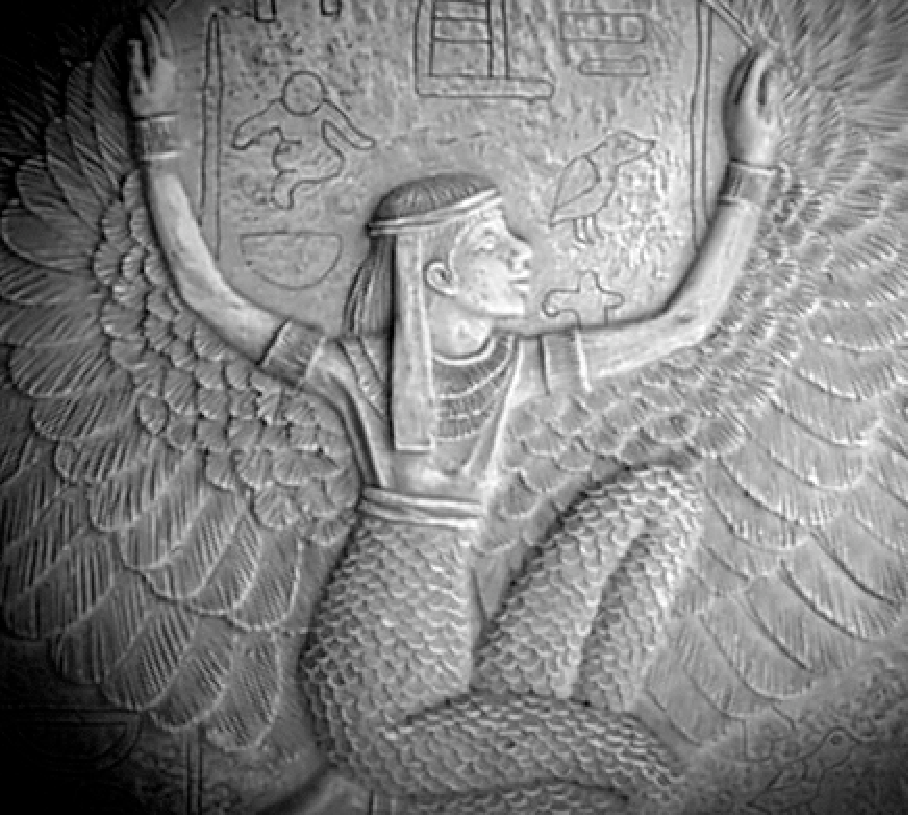
\includegraphics[width=1.5in]{isis1.pdf}
%%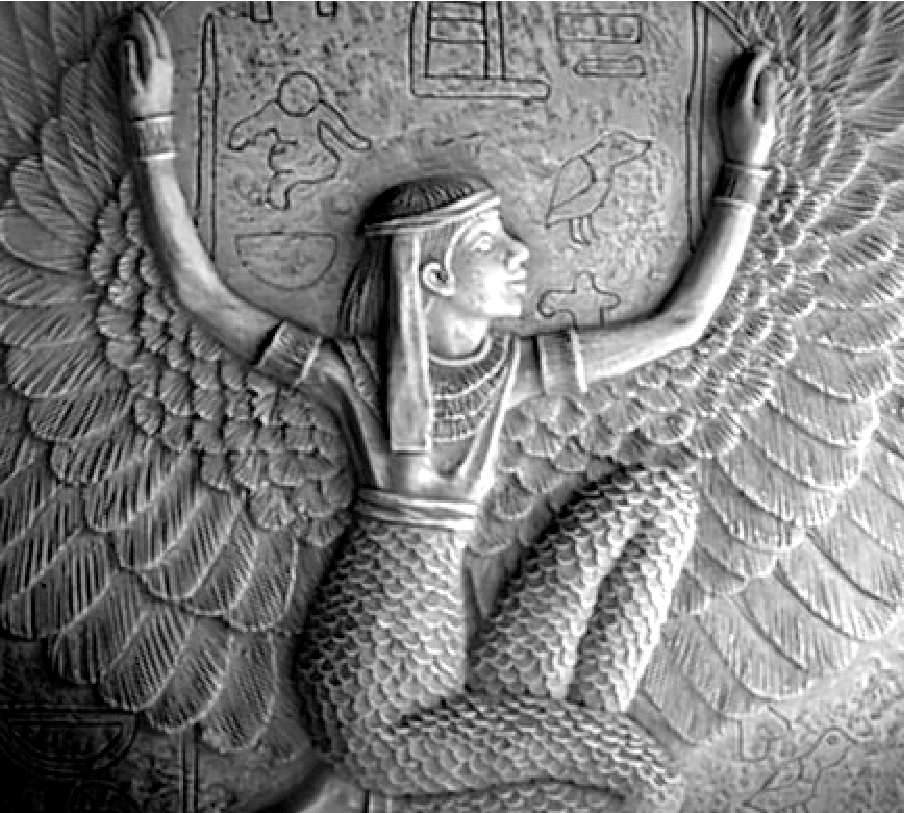
\includegraphics[width=1.5in]{isis2.pdf}
%%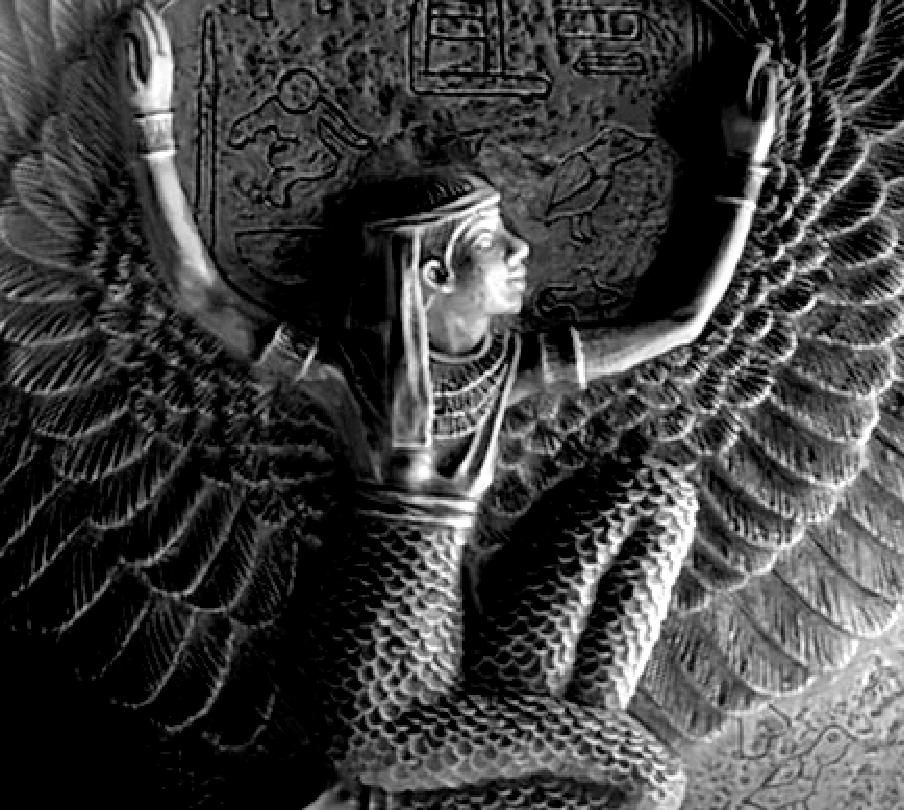
\includegraphics[width=1.5in]{isis3.pdf}
%%\end{center}

%\item Grid computing using modern video hardware\\
%Modern video cards for inexpensive consumer computers are 
%armed with powerful graphics processing units (GPU's) designed for
%fast rendering of 3D geometry. The research community has
%demonstrated how to exploit this extra computing power for
%non-graphics related applications. Certain classes of
%problems that involve computations on large structured grids
%are well suited to this heavily parallel, vector-based architecture.
%I am working with Ryan Tindall, who finished his Master's Degree in 
%December~2005 under my auspices, on using GPU hardware for simulating
%the propagation of electromagnetic waves.

%\end{enumerate}

%\pagebreak

\noindent{\large\bf Publications}

\begin{enumerate}

\item Wayne O. Cochran,
Recurrent Interpolation Surfaces,
{\em Proceedings of the Western Computer Graphics Symposium,}
March 2003, pp.~9--15.

\item Wayne. O. Cochran, R. R. Lewis, J. C. Hart,
The Normal of a Fractal Surface,
{\em The Visual Computer,} vol. 17, no. 4, April 2001, pp.~209--218.

\item Wayne O. Cochran,
Fractal Interpolation Surfaces for Digital Elevation Maps,
{\em Proceedings of the Western Computer Graphics Symposium,}
March 2001, pp.~8--14.

\item Wayne O. Cochran,
A Recurrent Modeling Toolset, Ph.D. dissertation.
Washington State University, December 1998.

\item
Wayne O. Cochran, John C. Hart, Patrick J. Flynn,
On Approximating Rough Curves with Fractal Functions,
{\em Proceedings of Graphics Interface,}
June 1998.

\item
J.C. Hart, P.J. Flynn, W.O. Cochran. 
Similarity Hashing: A Model-Based Vision Solution to the Inverse 
Problem of Recurrent Iterated Function Systems. 
{\em Fractals 5} April 1997, pp.~39-50.

\item
Wayne O. Cochran, John C. Hart, Patrick J. Flynn,
Hashing Fractal Functions
{\em Proceedings of the Western Computer Graphics Symposium,}
April 1997, pp.~69--78.

\item
Wayne O. Cochran, John C. Hart, Patrick J. Flynn,
Fractal Volume Compression,
{\em IEEE Transactions on Visualization and Computer Graphics}
2 (4),
%vol. 2, no. 4, 
December 1996, pp.~313--322.

\item
Wayne O. Cochran, John C. Hart, Patrick J. Flynn,
Similarity and Affinity Hashing,
{\em Proceedings of the Western Computer Graphics Symposium,}
March 1996, pp.~89--100.

\item
Wayne O. Cochran, J.C. Hart and P.J. Flynn. Recurrent Modeling. 
{\em Intel Forum: Enabling Live Media in Cyberspace,} 
invited poster. January 1996.

\item
Wayne O. Cochran, John C. Hart, Patrick J. Flynn,
Principal Component Classification for Fractal Volume Compression,
{\em Proceedings of the Western Computer Graphics Symposium,}
March 1995, \mbox{pp.~9--18}.

\end{enumerate}

%\vspace{0.25cm}
%\pagebreak

%\pagebreak

%\noindent{\large\bf Courses Taught}
%
%\begin{enumerate}
%\item Spring 2006, CptS 548, Advanced Computer Graphics, 3 credits, 3 %students.
%\item Spring 2006, CS 355, Programming Language Design, 3 credits, 
%    16 students.
%\item Fall 2005, CptS 442, Computer Graphics, 
%   3 credits, 9 students.
%\item Fall 2005, CptS 317, Automata and Formal Languages, 3 credits,
%   19 students.
%\item Spring 2005, CptS 548, Advanced Computer Graphics, 3 credits, 1 %student.
%\item Spring 2005, CS 355, Programming Language Design, 3 credits, 
%    13 students.
%\item Fall 2004, CptS 442, Computer Graphics, 
%   3 credits, 8 students.
%\item Fall 2004, CptS 317, Automata and Formal Languages, 3 credits,
%   13 students.
%\item Spring 2004, CptS 355, Programming Language Design, 3 credits, 
%    13 students.
%\item Fall 2003, CptS 442/542, Computer Graphics, 3 credits, 40 students.
%\item Fall 2003, CptS 317, Automata and Formal Languages, 3 credits,
%   20 students.
%\item Spring 2003, CptS 355, Programming Language Design, 3 credits, 
%    26 students.
%\item Spring 2003, CptS 548, Advanced Computer Graphics, 3 credits, 2 %students
%\item Fall 2002, CptS 442/542, Computer Graphics, 3 credits, 12 students.
%\item Fall 2002, CptS 317, Automata and Formal Languages, 3 credits, 
%  26 students.
%\item Spring 2002, CptS 355, Programming Language Design, 3 credits, 
%    13 students
%\item Fall 2001, CptS 442/542, Computer Graphics, 3 credits, 40 students.
%\item Spring 2001, CptS 460, Operating Systems, 3 credits, 10 students.
%\item Fall 2000, CptS 317, Automata and Formal Languages, 3 credits, 
%   10 students.
%\item Fall 2000, CptS 499, Special Problems, 2 credits, 5 students.
%\item Spring 2000, CptS 460, Operating Systems, 3 credits, 12 students.
%\item Spring 2000, CptS 499, Special Problems, 2 credits, 5 students.
%\item Fall 1999, CptS 317, Automata and Formal Languages, 3 credits, 
%   12 students.
%\item Spring 1999, CptS 455, Computer Networks, 3 credits,
%   80 students.
%\item Spring 1999, CptS 253, Java Programming Language, 3 credits, 
%   50 students.
%\item Fall 1998, EE 305, Introduction to Microprocessors, 2 credits,
%   20 students.
%\item Fall 1998, CptS 251, C Programming Language, 2 credits, 80 students.
%\item Fall 1998, CptS 252, Introduction to Windows Development Programming,
%  3 credits, 10 students.
%\end{enumerate}

%\vspace{0.25cm}

%\pagebreak

\noindent{\large\bf Graduate Student Advising}
\begin{itemize}
\item Jason Neufeld, (Current) MS Topic: {\em Tiling Techniques for Texture Maps.}
\item Michael Persons, MS May 2010.
  {\em Methods for Generating Wang Tiles.}
\item Gunay Uyan, MS December 2005. {\em Efficient Wang-Tiling and Real Time
   Rendering of Lambertian Reflectance Maps.}
\item Ryan Tindall, MS December 2005. {\em Graphics Hardware Acceleration
   of the Finite Difference Time Domain (FDTD) Algorithm.}
\end{itemize}

%\vspace{0.25cm}

%\noindent{\large\bf Graduate Student Committee Member}
%\begin{itemize}
%\item James Edwards, MS December 2005. {\em A Hardware
%    Implementation of a Multilevel B-Spline Shader.}
%\item Randolf Schwartz, MS May 2005. {\em MCNPVIZ: A Program for the
%    Interactive Display of Monte Carlo N-Particle Geometry.}
%\item Shuangshuang Jin, MS 2003, {\em A Comparison of
%    Algorithms for Vertex Normal Computation.}
%\item Masaki Kameya, PhD 2002, {\em A Smooth,
%   Efficient Representation of Reflectance.}
%\item Cheng-Chih Fan-Chiang. MS 2002, {\em Star-Flower
%   Subdivision.}
%\item Frank Taylor, MS 2001, {\em Enhancements to a 
%   Virtual Assembly Environment for Simulation of Heavy
%   Machinery Assembly.}   
%\item Nathan Carr, MS 2000, {\em Procedural Solid
%   Texture Mapping Using Existing Computer Graphics API's.}
%\item Shuyang Li, MS 2000, {\em Computing Reflectance
%   from Height Fields.}
%\end{itemize}

%\vspace{0.25cm}

%\noindent{\large\bf Software Disseminated}

%\begin{enumerate}
%\item Libraries for reading and viewing digital elevation maps.
%\item 2D image and 3D volumetric compression software using
%  DCT and fractal techniques.
%\end{enumerate}

%\pagebreak
%\vspace{0.25cm}

%\noindent{\large\bf Committees}
%
%\begin{itemize}
%\item 2010. (Chair) Graduate Studies Committee, 
%  School of Engineering and Computer Science.
%\item 2009-2010. WSUV Scholarship Committee.
%\item 2008. General Education Assessment Committee.
%\item 2007. General Education Studies Committee.
%\item 2004-2006. (Chair) Graduate Studies Committee, 
%  School of Engineering and Computer Science.
%\item 2005. Lower Division General Education 
%     Curriculum Committee, WSUV.
%\item 2004-2006. Undergraduate Studies Committee,
%  School of Engineering and Computer Science.
%\item 2004. Undergraduate Curriculum Committee,
%  School of Engineering and Computer Science.
%\item Faculty Search Committees, 2000, 2001, 2003, 2004, 2005.
%\item Network System Administrator Search Committee, 2000.
%\item 2000 -- 2002. Faculty Governance Committee.\\
%  Provides a formal, recognized structure through 
%  which faculty can have
%  direct input in administrative decision making.
%\end{itemize}

\vspace{0.25cm}

\noindent{\large\bf Consulting}

\begin{itemize}

\item Integrated Engineering Solutions, 
1610 NE Eastgate Blvd.
Suite 440
Pullman, WA 99163,
\verb@www.ie-sol.com.@
Designed and implemented a video stitching algorithm for
a stereo panorama camera system. The solution was
implemented using NVidia's CUDA parallel computing platform
for Telsa GPU-based systems.


\item GeoMonkey, Inc, 
5512 NE 109th Ct. Ste 101
Vancouver, WA 98662,
(360) 718-8120,
{\tt \verb@www.geomonkey.com@.}  
  Converted large KML polygonal datasets into a form used for
  fast multiresolution viewing in Google Maps.
  Also helped implement the {\tt MapWithUs GIS} iPhone app using Apple's core location technology
  and Google's map API.
\item Smith-Root Inc, 14014 NE Salmon Creek Avenue, Vancouver, WA 98686.\\
Helped design and port control software for an
electronic fish barrier. The system is now web based, and uses a 
client/server protocol for remote control.
\end{itemize}

%\vspace{0.5cm}
%\pagebreak


%\noindent{\large\bf Reviewer}
\noindent{\large\bf Professional Service}

\begin{itemize}
\item Paper Chair for Thirteen Annual {\em Consortium for Computing Sciences in Colleges} (CCSC)
Northwestern Regional Conference 2011. Responsible for collecting all submitted papers, procuring referees, and organizing the paper acceptance committee.
\end{itemize}

\noindent{Paper Referee for the following Journals and Conferences:}
\begin{itemize}
\item ACM SIGGRAPH
\item ACM Transactions on Graphics
\item IEEE Transactions on Visualization and Computer Graphics
\item IEEE Transactions on Pattern Analysis and Machine Intelligence
\item Information Processing Letters
\item Graphics Interface
\item IEEE Visualization
\item Shape Modeling International
\item International Conference on Cyberworlds
%   (2003, Singapore; 2004, Tokyo; 2005, Singapore).
%\item 2003 International Conference on Cyberworlds, 
%   December 3-5, 2003, Singapore.
%\item 2004 International Conference on Cyberworlds, 
%   November 10-20, 2004, Tokyo.
\end{itemize}

\vspace{0.25cm}

%\pagebreak

\noindent{\large\bf Awards}

\begin{itemize}
\item Curtis Fellowship, 1994, Washington State University.
\item Phi Beta Kappa, 1990, Alpha Chapter, University of Washington.
\item Deans List, 1990, University of Washington.
\item Golden Key National Honor Society, 1990, University of Washington.
\end{itemize}

%\vspace{0.25cm}

%\pagebreak

%\noindent{\large\bf Other Activities}\\
%\noindent{\large\bf Professional Service}\\

%\noindent{WSU Linux Users Group, co-founder:}
%\begin{itemize}
%\item Faculty Advisor (1998--1999)
%\item President (1997--1998) 
%\item Treasurer (1994--1997),
%\end{itemize}

%\noindent{1995 {\em SIGGRAPH} student volunteer.}\\

%\noindent{\large\bf Courses Able to Teach}
%
%\begin{itemize}
%\item Programming Languages (C, C++, Java, Common Lisp, Ada, Assembly, \ldots)
%\item Computer Graphics
%\item Computer Networks
%\item Distributed Computing
%\item Operating Systems
%\item Compiler Design
%\item Program Design, Data Structures
%\item Theory of Computation
%\item User Interface Programming (Windows, X Window System, \ldots)
%\item Numerical Computation, Numerical Analysis
%\item Mathematics (Calculus, Linear Algebra, \ldots)
%\end{itemize}


%\vspace{0.25cm}

%\noindent{\large\bf Computer Skills}

%\begin{itemize}
%\item Programming in the UNIX and the X Window System environment.
%\item UNIX and X Window System administration.
%%\item MS Windows programming.
%\item Distributed and threaded computing (PVM, Posix threads, \ldots).
%\item High and low level graphics programming (OpenGL, \ldots).
%\item Programming languages: C, C{\small++}, Java, Common Lisp, 
%       Assembly.
%\end{itemize}

\vspace{0.25cm}

\noindent{\large\bf References}\\

Charles R. Lang\\ 
Associate Professor \\
School of Engineering and Computer Science \\
Washington State University Vancouver \\
14204 NE Salmon Creek Avenue \\
Vancouver, Washington 98686-9600 \\
\verb$dick_lang@vancouver.wsu.edu$ \\
(360) 546-9632.\\

Roger C. Ray\\
Principal Engineer, Intel (retired)\\
{\tt roger@anastasia.com} \\
(503) 292-1476.\\
 
John C. Hart\\
Professor\\
Department of Computer Science\\
University of Illinois\\
3233 Siebel Center \\
201 N. Goodwin \\
Urbana, IL 61801 \\
%{\tt jch@cs.uiuc.edu} \\
{\tt jch@illinois.edu} \\
(217) 333-8740 \\

%Patrick J. Flynn, Associate Professor,
%Department of Computer Science and Engineering,
%University of Notre Dame,
%384 Fitzpatrick Hall of Engineering,
%Notre Dame, Indiana 46556,
%(219) 631-8803.\\

%Phil Smith, President,
%Raster Graphics Inc,
%1804 SE First Street,
%Redmond, OR 97756,
%(541) 923-5530.

\end{document}

